%%%%%%%%%%%%%%%%%%%%%%%%%%%%%%%%%%%%%%%%%%%%%%%%%%%%%%%%%% 
\section{実行実験}\label{chap:experiment}
%%%%%%%%%%%%%%%%%%%%%%%%%%%%%%%%%%%%%%%%%%%%%%%%%%%%%%%%%% 

本章では,前章で提案した3つの符号化
\textsf{undirected},\textsf{directed},\textsf{acyclicity}
の性能を評価するために実行実験を行った.
%
実験に使用したベンチマーク問題集(計1008問)は,以下の通りである.
\begin{itemize}
\item \textsf{fhcp} (1001問)\\
  Jerzy Filar と Vladimir Ejov が主導する
  チームプロジェクト Flinders Hamiltonian Cycle Project
%  \footnote{\href{https://sites.flinders.edu.au/flinders-hamiltonian-cycle-project/}{リンク}}
%  \footnote{\url{https://sites.flinders.edu.au/flinders-hamiltonian-cycle-project/}}
  が提供するハミルトン閉路問題のグラフインスタンス.\cite{haythorpe19:fhcp}
\item \textsf{grid} (6問)\\
  $2N+1$次の正方グリッドグラフのインスタンス($3\leq N\leq 8$).
\item \textsf{usmap} (1問)\\
  図~\ref{fig:USmap}に示されたグラフ.
  D.~E~.Knuth の教科書
  The Art of Computer Programming~\cite{Knuth:TAOCP:SAT}
  に記載されている最短ハミルトン路問題の例.
\end{itemize}

使用した ASP システムは{\clingo}のバージョン5.5.0である.
実験環境は,Mac mini Intel Corei7 3.2GHz 64GBメモリである.

%%%%%%%%%%%%%%%%%%%%%%%%%%%%%%%%%%%%%%%%%%%%%%%%%%%%%%%%%%
\subsection{ハミルトン閉路問題の実験結果}
%%%%%%%%%%%%%%%%%%%%%%%%%%%%%%%%%%%%%%%%%%%%%%%%%%%%%%%%%%

%%%%%%%%%%%%%%%%%%%%%%%%%%%%%%%%%%%%%%%%%%%%%%%
\begin{table}[t]\scriptsize
  \centering
  %\tabcolsep = 0.8mm
  \renewcommand{\arraystretch}{1.2}
  \begin{tabular}{lr|rrr}
    問題サイズ & 問題数 & \textsf{undirected} & \textsf{directed} & \textsf{acyclicity}\\
   \hline
    $\:\:\:\:\:\,\, 0 \leq |V| < 1000$     & 171   & 156   & \alert{171}   & 156  \\ %
    $1000 \leq |V| < 2000$  & 165   & 120   & \alert{159}   & 121  \\
    $2000 \leq |V| < 3000$  & 177   & 125   & \alert{163}   & 80   \\
    $3000 \leq |V| < 4000$  & 185   & 104   & \alert{147}   & 48   \\
    $4000 \leq |V| < 5000$  & 128   & 92    & \alert{106}   & 30   \\
    $5000 \leq |V| < 6000$  & 80    & 63    & \alert{70}    & 21   \\
    $6000 \leq |V| < 7000$  & 55    & 39    & \alert{41}    & 20   \\
    $7000 \leq |V| < 8000$  & 28    & 12    & \alert{15}    & 4    \\
    $8000 \leq |V| < 9000$  & 10    & 2     & \alert{5}     & 1    \\
    $9000 \leq |V| < 10000$  & 2     & \alert{2}     & \alert{2}     & 1    \\
   \hline
    合計 & 1001 & 715   & \alert{879}   & 482  
  \end{tabular}
  \vskip .5em
%  \caption{ハミルトン閉路問題: 解けた問題数}
  \label{sat_table}
\end{table}
%label{sat_table}
%%%%%%%%%%%%%%%%%%%%%%%%%%%%%%%%%%%%%%%%%%%%%%%

%%%%%%%%%%%%%%%%%%%%%%%%%%%%%%%%%%%%%%%%%%%%%%%
\begin{figure}[tb]
\begin{center}
  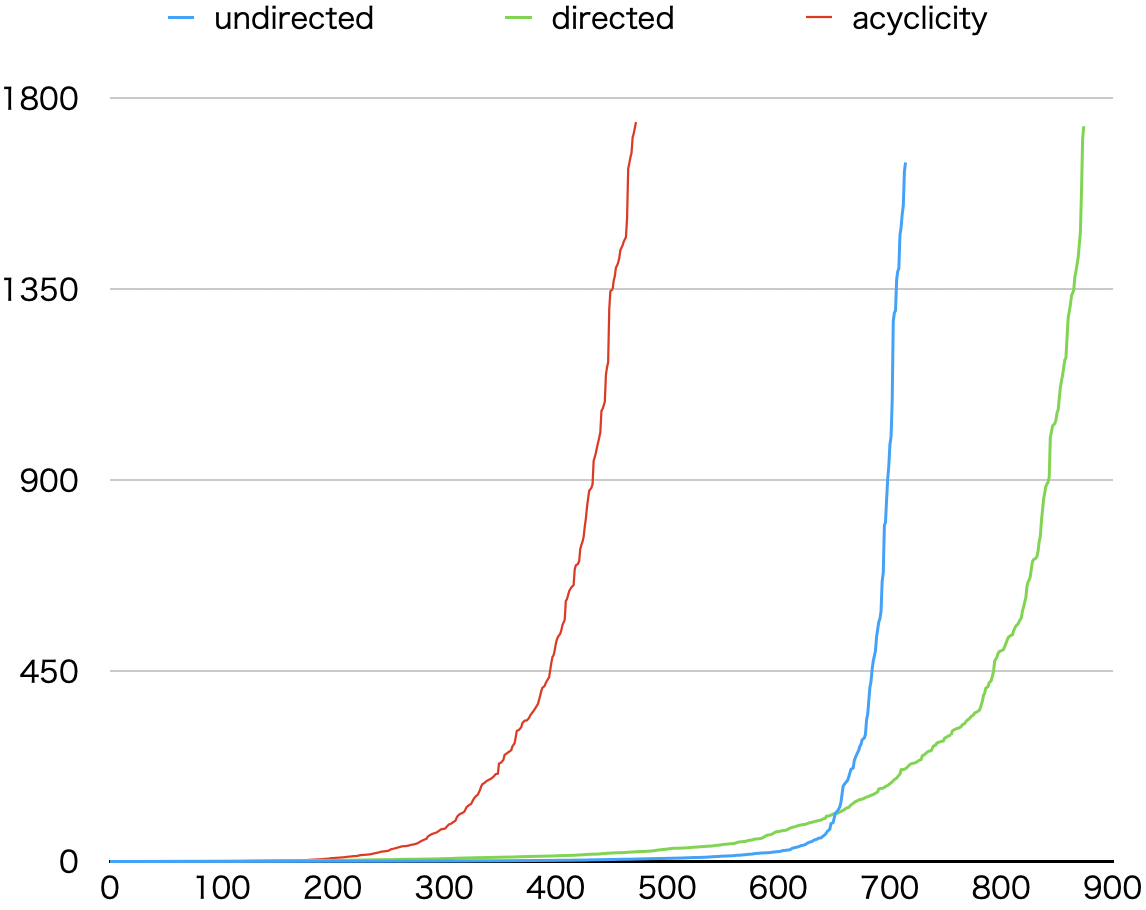
\includegraphics[width=0.8\linewidth]{fig/cactus_fhcp.png}
\caption{ハミルトン閉路問題: カクタスプロット}
\label{cactus}
\end{center}
\end{figure}
%%%%%%%%%%%%%%%%%%%%%%%%%%%%%%%%%%%%%%%%%%%%%%%


%--
本節では,ハミルトン閉路問題の実験結果について述べる.
{\clingo}のオプションは\textit{trendy}を使用し,一問あたりの時間制限を30分とした.
ベンチマーク問題は,\textsf{fhcp}の1001問である.

%--
表~\ref{sat_table}に,各符号化で解けた問題数を,問題の頂点数毎に示す.
左から,問題の頂点数,問題数,各符号化で解けた問題数を示している.
%
解けた問題数は,
\textsf{undirected}符号化が715問,
\textsf{directed}符号化が875問,
\textsf{acyclicity}符号化が473問であり,
\textsf{directed}がもっとも多くの問題を解いた.
\textsf{directed}は,どの頂点数においても同様に,
安定した性能の良さを示した.
図~\ref{cactus}に,カクタスプロットを示す.
縦軸は問題を解くのに要した CPU 時間,横軸は解けた問題数を表す.
グラフが右によるほど多くの問題を解けたことを示し,
下によるほどより速く解けたことを示す.
図~\ref{cactus}より,\textsf{directed}符号化が,
他の2つの符号化と比較して,より多くの問題を高速に解いていることが確認できた.
%% しかし,一部\textsf{undirected}符号化が\textsf{directed}符号化を下回る
%% 部分が確認できる.
%% 実際に,一部の問題では\textsf{undirected}符号化が
%% \textsf{directed}符号化よりも高速に解いていた.

%%%%%%%%%%%%%%%%%%%%%%%%%%%%%%%%%%%%%%%%%%%%%%%%%%%%%%%%%%
\subsection{最短ハミルトン路問題}
%%%%%%%%%%%%%%%%%%%%%%%%%%%%%%%%%%%%%%%%%%%%%%%%%%%%%%%%%%

%%%%%%%%%%%%%%%%%%%%%%%%%%%%%%%%%%%%%%%%%%%%%%%
\begin{table}[htbp]
  \caption{実験結果2-1:trendy}
  \label{min_table_tr}
  \centering
  \begin{tabular}{|l|rrr|}
    \hline
    Instance&undirected&directed&acyclicity \\
    \hline
    grid5&50,656*&50,656*&50,656* \\
    grid6&68,656*&68,656*&68,656* \\
    grid7&91,822*&91,822*&91,822* \\
grid8&113,250&\textcolor{red}{112,916}&113,277 \\
grid9&\textcolor{red}{142,502}&143,326&143,660 \\
grid10rc&\textcolor{red}{172,703}&174,866&175,999 \\
grid11&\textcolor{red}{200,399}&204,456&200,638 \\
grid12&\textcolor{red}{231,278}&239,275&232,012 \\
grid13&\textcolor{red}{276,692}&276,926&276,899 \\
grid14&317,617&\textcolor{red}{317,144}&317,676 \\
grid15&\textcolor{red}{375,906}&376,809&376,210 \\
grid16&421,249&\textcolor{red}{419,737}&423,753 \\
US48&11,698*&11,698*&11,698* \\
    \hline
  \end{tabular}
\end{table}
%\label{min_table_tr}
%%%%%%%%%%%%%%%%%%%%%%%%%%%%%%%%%%%%%%%%%%%%%%%

%--
本節では,最短ハミルトン閉路問題の実験結果について述べる.
{\clingo}のオプションは\textit{trendy}を使用し,
一問あたりの時間制限を3時間とした.
ベンチマーク問題は,\textsf{grid}と\textsf{usmap}の合計7問である.

%--
表\ref{min_table_tr}に,各符号化で得られた最適値と最良値を示す.
各問題毎に,最も良かった値を赤字で示している.
*マークは,最適値を表している.
最適値と最良値の数は,
\textsf{undirected}符号化が5問,
\textsf{directed}符号化が3問,
\textsf{acyclicity}符号化が3問であり,
\textsf{undirected}符号化の優位性が確認できた.
なお,全ての符号化で最適値を求めることのできた2問においても,
\textsf{undirected}符号化がもっとも高速に解を求めていた.

%%%%%%%%%%%%%%%%%%%%%%%%%%%%%%%%%%%%%%%%%%%%%%%%%%%%%%%%%%
\subsection{コスト制約付きハミルトン路問題}
%%%%%%%%%%%%%%%%%%%%%%%%%%%%%%%%%%%%%%%%%%%%%%%%%%%%%%%%%%

%%%%%%%%%%%%%%%%%%%%%%%%%%%%%%%%%%%%%%%%%%%%%%%
\begin{table*}[tb]\footnotesize
  \tabcolsep = 2mm
  %\renewcommand{\arraystretch}{1.0}
  \vskip .5em
  \centering
  \begin{tabular}{lr|rrr}
    \hline
    閾値(倍率)    &	解の総数 & \textsf{undirected} & \textsf{directed} & \textsf{acyclicity} \\
    \hline
    11698(1.00)   &	1      &\textbf{2.979} & 7.531 & 4.586	\\
    11814(1.01)   &	8      &5.587  & 15.322	& \textbf{5.250}	\\
    11931(1.02)   &	28     &\textbf{3.243}& 18.600	& 3.578	\\
    12282(1.05)   &	388    &10.003&19.818	& \textbf{6.296}	\\
    12867(1.10)   &	16,180  &16.548& 28.555	& \textbf{9.764}\\
    14037(1.20)   &	939,209 &48.262       &40.717	& \textbf{26.837}\\
    15207(1.30)   &	4,525,541&88.172      &55.276	& \textbf{42.037}\\
    16377(1.40)   &	6,702,964&99.154       &47.647	& \textbf{40.640}	\\
    17547(1.50)   &	6,876,526&95.390       &45.265	& \textbf{38.411}	\\
    18716(1.60)   &	6,876,928&98.937       &49.138	& \textbf{40.748}	\\
    \hline
    平均CPU時間 &   & 46.8275 & 32.7869  & \textbf{21.8147}\\\hline
%    Best    &   & 2 & 0 & \textbf{8} \\ \hline
  \end{tabular}
  \vskip .5em
  \caption{コスト制約付きハミルトン路問題: 解の全列挙に要した CPU 時間}
  \label{cost_table}
\end{table*}
%\label{cost_table}
%%%%%%%%%%%%%%%%%%%%%%%%%%%%%%%%%%%%%%%%%%%%%%%

%--
本節では,第~\ref{chap:background}章でも説明した
コスト制約付きハミルトン路問題(全列挙)の実験結果について述べる.
{\clingo}のオプションは\textit{crafty}を使用し,
一問あたりの時間制限を3時間とした.
ベンチマーク問題は,D.~E~.Knuth の教科書
The Art of Computer Programming~\cite{Knuth:TAOCP:SAT}
に記載されているグラフを使用した(図~\ref{fig:USmap}参照).
このグラフは,米国本土48州の隣接関係を表しており,
頂点数は48,辺の数は105である.
この問題の最短距離は 11698 である(表~\ref{min_table_tr}参照).
今回の実験では,
コスト制約を最短距離のN倍以下
($N=1.00,1.01,1.02,1.05,1.1,1.2,1.3,1.4,1.5,1.6$)として,解の全列挙を
行った.

%--
表~\ref{cost_table}に,各符号化が解の全列挙に要した CPU 時間を示す.
表の1列目はコスト制約の閾値と最短距離からの倍率,2列目は解の総数を表している.
各閾値毎に,最も良かった値を赤字で示している.
表より,
\textsf{acyclicity}符号化が,他の符号化と比較して,より多くの問題を
高速に解いていることがわかる.また,平均CPU時間も最も短い.
%%%%%%%%%%%%%%%%%%%%%%%%%%%%%%%%%%%%%%%%%%%%%%%%%%%%%%%%%%

%%% Local Variables:
%%% mode: latex
%%% TeX-master: "paper"
%%% End:
